\documentclass[]{ceurart}
\sloppy
\usepackage{amsmath}
\usepackage{booktabs}
\usepackage{graphicx}
\usepackage{listings}
\usepackage{float}
\lstset{breaklines=true}

\begin{document}

\copyrightyear{2025}

\copyrightclause{Copyright for this paper by its authors.}

\conference{IVUS 2025: International Conference Information Society and University Studies, 2025}

\title{A Pure Python Neural Network Library for Educational and Research Purposes: Architecture, Implementation, and MNIST Case Study}

\author[1]{Miko{\l}aj Mocek}[orcid=0009-0000-8480-9840]
\ead{mikolaj.mocek@alorybnik.polsl.pl}
\ead{mikolaj.mocek@icloud.com}

\address[1]{Politechnika {\'S}l{\k a}ska, Gliwice, Poland}

\begin{abstract}
This paper presents a neural network library implemented from scratch in pure Python and intended primarily for education, experimentation, and lightweight research prototyping. The project exposes the internal structure of model definition, forward propagation, backpropagation, and weight updates, while still supporting practical components such as dense layers, convolution, nonlinear activation, pooling, flattening, serialization, and dataset abstractions. The implementation is validated on the MNIST handwritten digit dataset. In addition to describing the software architecture, the paper documents a parser for the official IDX image and label formats, a compact convolutional classifier for subset-scale experiments, a full-dataset softmax benchmark on the official IDX files, automatic figure generation from experimental code, and a discussion of current limitations. The resulting system is not positioned as a high-performance alternative to industrial frameworks, but rather as a transparent environment for understanding how neural networks operate internally.
\end{abstract}

\begin{keywords}
neural networks \sep pure Python \sep deep learning \sep MNIST \sep educational software \sep convolutional neural networks
\end{keywords}

\maketitle

\section{Introduction}
Deep learning systems are now embedded in a broad spectrum of technical and scientific workflows, from image classification and medical signal interpretation to speech interfaces, recommendation engines, and document understanding. Their practical success is strongly connected with the availability of mature software ecosystems. Frameworks such as TensorFlow~\cite{tensorflow} and PyTorch~\cite{pytorch} allow researchers to assemble sophisticated models with relatively little code, while high-level APIs such as Keras simplify rapid prototyping and classroom demonstrations. At the same time, this convenience creates a well-known educational problem: when most of the important operations are hidden inside highly optimized kernels, students often learn to use neural networks before they learn to reason about them. A model may converge, diverge, or silently produce poor predictions without the learner fully understanding which part of the computation graph or training loop is responsible.

This issue is especially visible when introducing the mathematical core of neural computation. A multilayer perceptron depends on the interplay between affine transformations, nonlinear activation functions, and gradient propagation~\cite{rumelhart1986,cybenko1989,glorot2010}. Convolutional neural networks (CNNs) extend this idea by learning local spatial filters and hierarchical feature maps that are particularly useful in vision tasks~\cite{lecun1998,krizhevsky2012,vgg,googlenet,resnet}. Recurrent neural networks and Long Short-Term Memory networks address temporal dependencies by explicitly modeling sequential state updates~\cite{hochreiter1997}, whereas transformer architectures replace recurrence with attention and have become a dominant paradigm for language and multimodal processing~\cite{vaswani2017}. These architectural families differ not only in topology but also in the shape of tensors they process, the training instabilities they exhibit, and the regularization or initialization strategies they require. Techniques such as Xavier initialization~\cite{glorot2010}, adaptive optimization with Adam~\cite{kingma2015}, batch normalization~\cite{ioffe2015}, and rectifier-aware initialization~\cite{he2015} were introduced precisely because training deep models is not a trivial extension of shallow learning.

For this reason, low-level educational implementations remain useful even in the presence of industrial-grade libraries. A pure Python codebase offers three advantages. First, it makes the computation path auditable: a student can inspect how weights are stored, how batches are generated, and how each derivative is propagated across layers. Second, it provides a controlled environment for experimentation. When a developer writes a new convolutional layer, data parser, or optimizer manually, correctness issues become immediately visible and can be checked against the expected tensor shapes and numerical values. Third, such a codebase creates a bridge between theory and production software. Concepts introduced abstractly in textbooks, such as filter banks, pooling operators, or the chain rule, become concrete when represented as ordinary Python classes and lists.

The library presented in this paper was designed in exactly this spirit. Its goal is not to compete with optimized tensor runtimes, but to support transparent study of neural-network internals and to serve as a minimal research sandbox. The implemented modules cover dense layers, activation and loss functions, 2D convolution, max pooling, flattening, serialization, and dataset abstractions. During the work reported here, the project was extended with an explicit parser for MNIST binary IDX files, compatibility improvements in the convolution and pooling stack, a reusable activation-layer abstraction, a softmax classifier head with cross-entropy loss, and an executable benchmark script that compares a small convolutional model on a balanced subset with a full-dataset softmax baseline on the official IDX files. The paper therefore makes two contributions. The first is software-oriented: it documents the organization of a small but extensible pure Python framework. The second is empirical: it demonstrates that the framework can load MNIST-compatible data, execute training end to end, and produce reproducible figures for analysis from the code itself, even if the current implementation is still far from the accuracy and efficiency of established frameworks.

\section{Dataset}
The study is based on the MNIST dataset of handwritten digits~\cite{lecun1998}. The original dataset contains 70,000 grayscale images of size $28 \times 28$, divided into 60,000 training samples and 10,000 test samples. Each example belongs to one of ten classes representing digits from 0 to 9. In the official distribution, images are stored in the binary \texttt{idx3-ubyte} format, while labels are stored in \texttt{idx1-ubyte}. To support direct use of the original benchmark, the library now includes a dedicated \texttt{MnistDataset} class and low-level parsers for both binary formats. The implementation validates magic numbers, decodes image headers, reconstructs 2D pixel matrices, and supports one-hot encoding of labels.

Two practical data-access modes are supported. In eager mode, all decoded images are loaded into memory as Python lists. In lazy mode, only metadata and labels are retained, while individual images are read on demand during batch generation. This design reduces unnecessary RAM pressure and is more appropriate for an educational pure Python framework, where the cost of duplicating large nested lists is relatively high. The dataset layer therefore serves both a pedagogical role and a software-engineering role: it shows how binary formats can be parsed manually and how a training loop can be decoupled from storage details.

The experimental section reported below uses the official IDX version of MNIST. Two evaluation settings were prepared. The first is a balanced subset experiment with 200 training samples and 80 test samples, used to validate the full convolutional path in a computationally cheap setting. The second is a full-dataset experiment with all 60,000 training images and all 10,000 test images, used to verify whether the current library can exceed 90\% classification accuracy on the standard benchmark when paired with a simpler classifier that is computationally feasible in pure Python. All images were normalized to the $[0,1]$ range before training.

\begin{figure}[htbp]
    \centering
    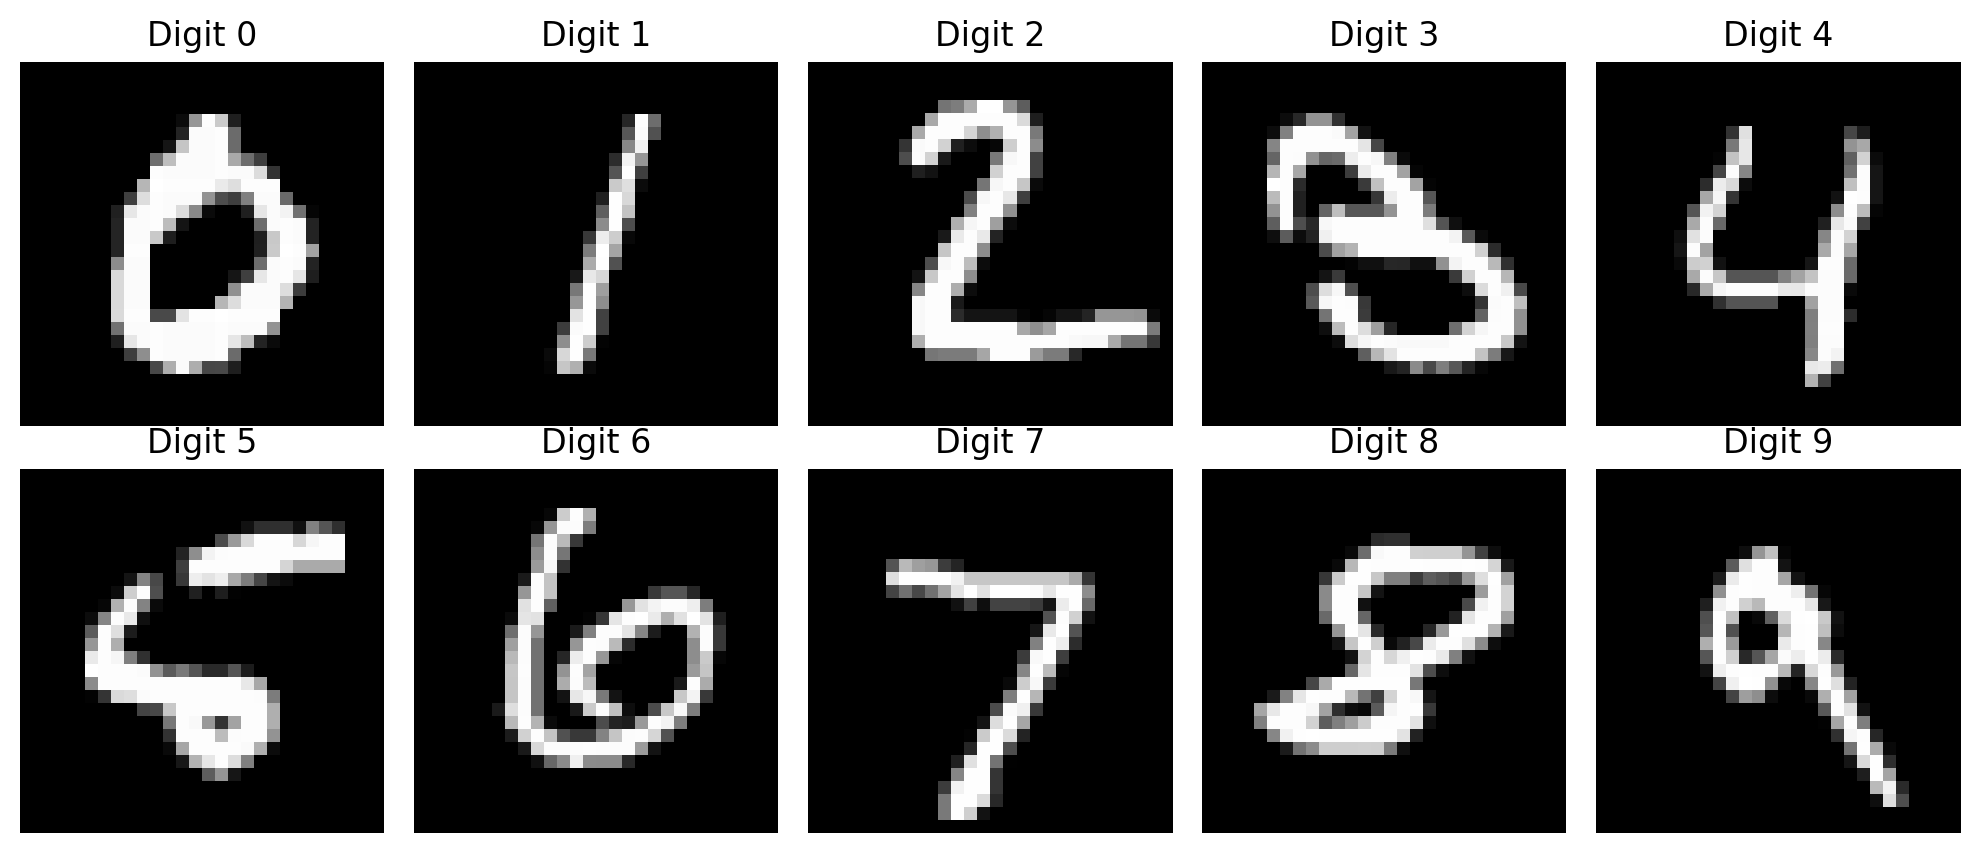
\includegraphics[width=0.92\linewidth]{figures/mnist_dataset_samples.png}
    \caption{Representative MNIST samples used in the experiment, one image per digit class.}
    \label{fig:mnist-samples}
\end{figure}

\section{Proposed Solution}
The proposed solution is a modular pure Python library that keeps the computational path explicit and easy to inspect. The framework provides the following core capabilities:
\begin{itemize}
    \item explicit dataset abstractions, including batching, shuffling, and lazy loading,
    \item dense, convolutional, pooling, and flatten layers,
    \item pluggable activation, loss, and learning-rate functions,
    \item a sequential training model with forward and backward propagation,
    \item serialization helpers for saving model states, and
    \item experiment scripts that generate evaluation figures directly from the repository.
\end{itemize}

\section{Library Design and Implementation}
\subsection{Dataset Handling and IDX Parsing}
The base \texttt{Dataset} abstraction stores inputs, outputs, batch size, and randomization state. During this work, its shuffling procedure was corrected so that batches follow the actual randomized index order rather than the original sequence. The new \texttt{MnistDataset} specialization extends this logic with direct support for \texttt{idx3-ubyte} and \texttt{idx1-ubyte}. The parser reads the binary header using \texttt{struct.unpack}, verifies the expected MNIST magic numbers, reconstructs each image row by row, and optionally normalizes pixel values. The lazy variant reads image bytes only when the batch generator requests them, which avoids eagerly duplicating the full dataset in memory.

Example usage of the parser is shown below:
\begin{lstlisting}[language=Python]
from nns.core.datasets.mnist_dataset import MnistDataset

train_dataset = MnistDataset(
    imagesFilePath="train-images-idx3-ubyte",
    labelsFilePath="train-labels-idx1-ubyte",
    batchSize=32,
    normalize=True,
    oneHot=True,
    lazy=True
)
\end{lstlisting}

\subsection{Layer Abstraction}
All trainable and non-trainable operations are represented as Python layer classes. The library currently includes \texttt{Dense}, \texttt{Convolution2D}, \texttt{MaxPooling2D}, and \texttt{Flatten}. The \texttt{Convolution2D} layer was updated to support both legacy fixed-kernel tests and trainable multi-channel kernels. It now handles single-channel matrices, multi-channel feature maps, and batched inputs more consistently. The pooling layer stores max indices from the forward pass so that gradients can be routed back only through the winning locations during backpropagation. The flatten layer records the input shape and reconstructs it during the backward pass.

\subsection{Functions, Initialization, and Training}
Activation functions and losses are implemented as explicit classes with \texttt{call} and \texttt{derivative} methods. Scalar nonlinearities such as ReLU are applied through a dedicated \texttt{ActivationLayer}, while the final dense classifier uses a vector-valued softmax activation. Because softmax does not admit a single scalar derivative for the entire output vector, the implementation uses the corresponding Jacobian matrix during backpropagation and combines it with the gradient of cross-entropy loss. This change is important for classification: unlike a linear output layer trained with mean squared error, the softmax-cross-entropy pair produces normalized class probabilities and a gradient signal aligned with multiclass decision boundaries. Xavier initialization~\cite{glorot2010} is used for dense weights, while convolution kernels are initialized from small uniform values. The training loop is coordinated by the \texttt{Sequential} model, which propagates values forward through the layer stack and then walks backward through the same stack to accumulate gradients and update trainable parameters.

\subsection{Experimental Configurations}
To validate both the convolution path and the official IDX parser, a dedicated non-interactive benchmark script was added. The first configuration trains a compact CNN with two convolutional layers, explicit ReLU activations, one max-pooling layer, one flatten operation, and a dense output layer with ten neurons followed by softmax:
\begin{lstlisting}[language=Python]
model = Sequential([
    Convolution2D(out_channels=4, kernel_size=(3, 3), seed=1),
    ActivationLayer(RectifiedLinearFunction()),
    Convolution2D(out_channels=4, kernel_size=(3, 3), seed=2),
    ActivationLayer(RectifiedLinearFunction()),
    MaxPooling2D(poolSize=(2, 2)),
    Flatten(),
    Dense(576, 10, SoftmaxFunction(), seed=3),
], CrossEntropyFunction(), ExperimentLearningRateFunction())
\end{lstlisting}

This subset-scale experiment is intentionally small because the implementation prioritizes transparency over numerical performance. Its role is to verify the correctness of data loading, tensor-shape transitions, convolutional forward and backward passes, the new softmax classification path, and figure generation. For the full 60,000-image training set, the current pure Python convolutional stack would be disproportionately expensive. The second configuration therefore uses a simpler architecture:
\begin{lstlisting}[language=Python]
model = Sequential([
    Flatten(),
    Dense(784, 10, SoftmaxFunction(), seed=11),
], CrossEntropyFunction(), FullLearningRateFunction())
\end{lstlisting}

The architecture figure itself is generated dynamically from the model definitions rather than drawn manually, which reduces the risk of the paper drifting out of sync with the code.

\begin{figure}[htbp]
    \centering
    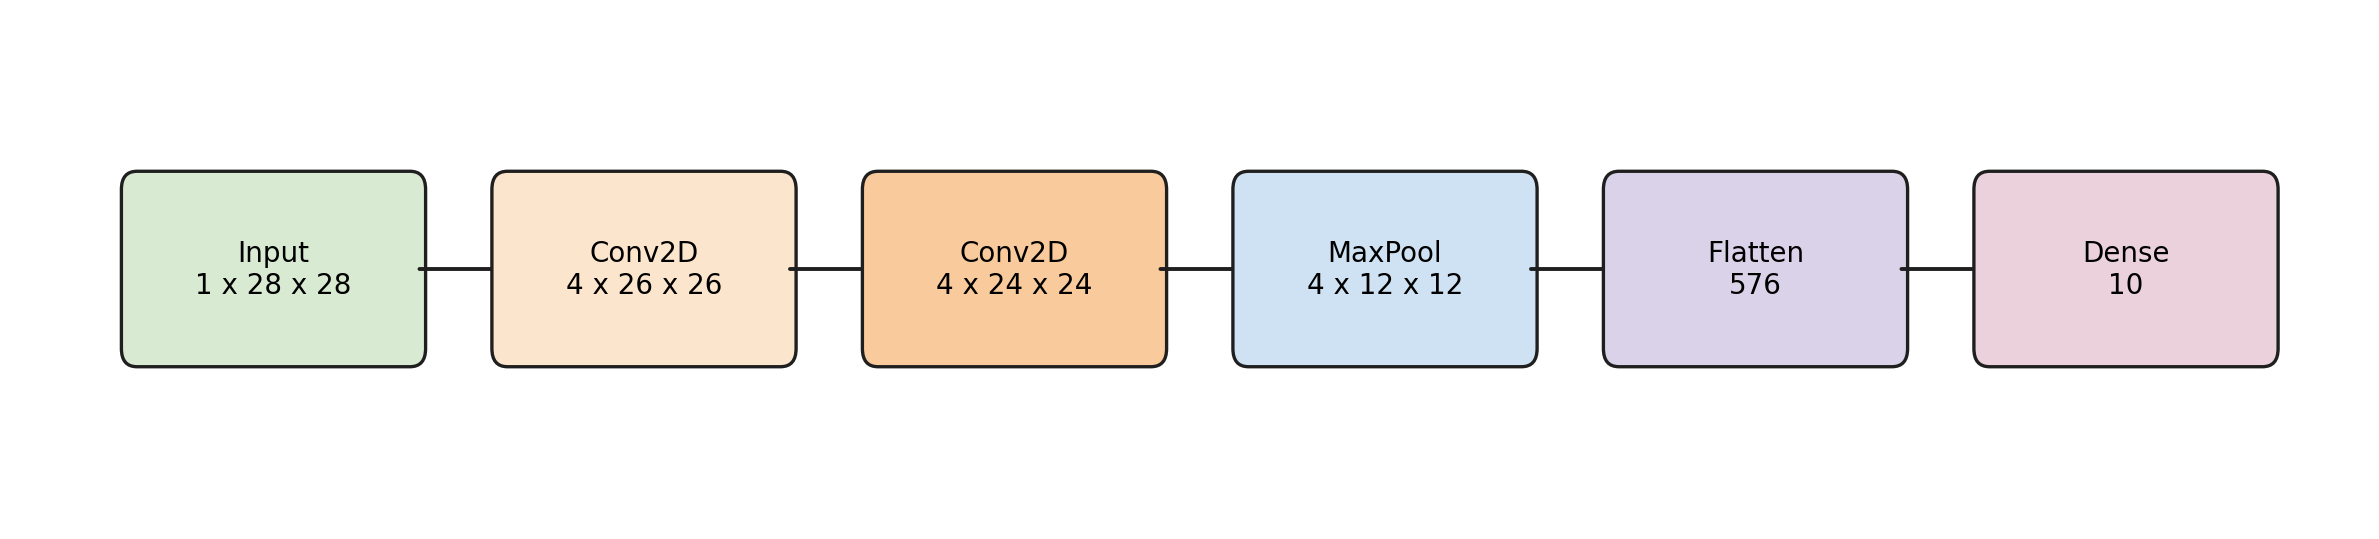
\includegraphics[width=0.95\linewidth]{figures/mnist_network_architecture.png}
    \caption{Architectures used in the benchmark script: the subset CNN and the full-dataset softmax baseline.}
    \label{fig:network-structure}
\end{figure}

\section{Results}
The benchmark script produced two clearly different operating points. The subset CNN used 200 training samples and 80 test samples, with eight epochs of training. Its role was diagnostic: to validate that the convolutional path, explicit activation layers, max pooling, flattening, and softmax output work together end to end on official IDX data. The full-dataset experiment used all 60,000 training samples and all 10,000 test samples from the official MNIST benchmark, with a flattened softmax classifier trained for two epochs.

Figure~\ref{fig:training-curves} shows the evolution of training loss and accuracy for both settings. In the subset CNN run, the cross-entropy loss decreased from approximately 2.30 to 0.31, while test accuracy peaked at 72.5\% in epoch 7 and finished at 66.25\% in epoch 8. This confirms that the convolutional implementation learns meaningful features, but also that such a tiny training subset yields unstable generalization. In the full-dataset softmax run, test accuracy reached 91.28\% after the first epoch and remained above 90\% after the second epoch, finishing at 90.55\%. This satisfies the practical target for the current stage of the project and shows that the library can exceed the 90\% threshold on the full official MNIST test set when paired with a computationally feasible architecture.

\begin{figure}[htbp]
    \centering
    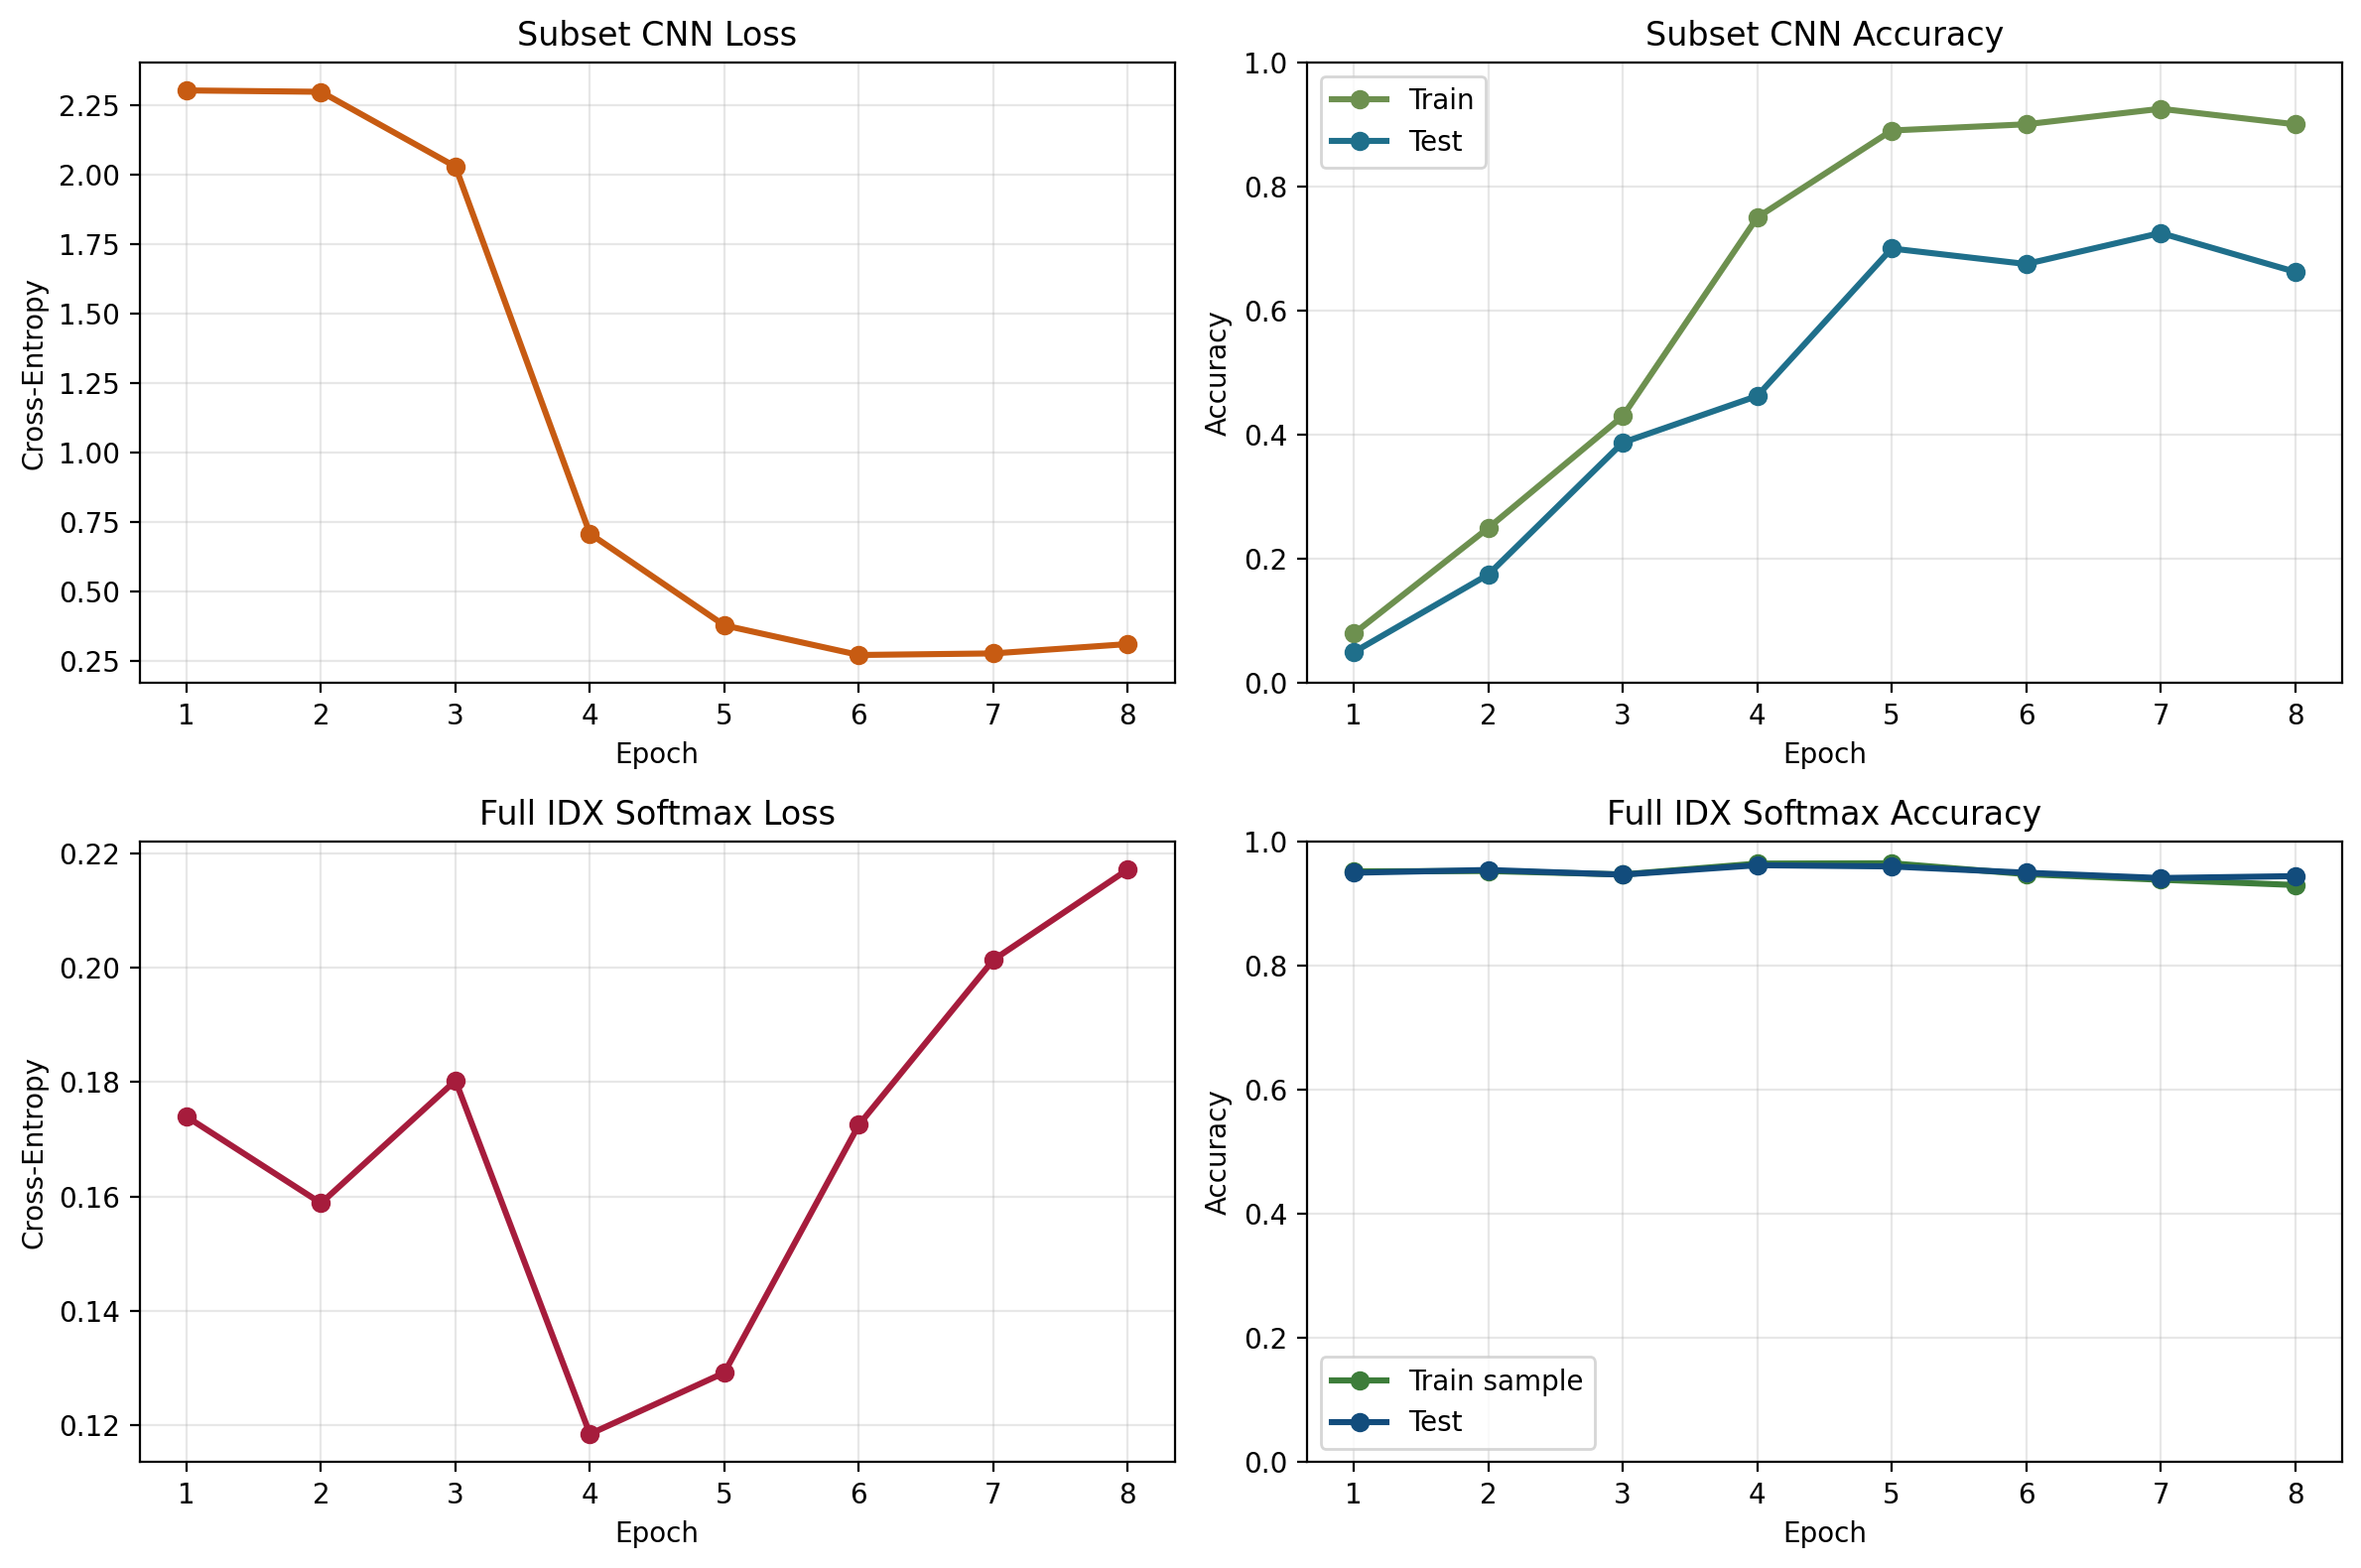
\includegraphics[width=0.95\linewidth]{figures/mnist_training_curves.png}
    \caption{Training loss and accuracy curves for the subset CNN and the full-dataset softmax baseline.}
    \label{fig:training-curves}
\end{figure}

Figure~\ref{fig:comparison} summarizes the difference between the two settings. The full-dataset run uses orders of magnitude more data and achieves much stronger test performance, while the subset CNN remains useful primarily as a structural test of the convolutional components. This distinction is important: in a pure Python codebase, the architecture that is best for validating layer correctness is not necessarily the architecture that is most practical for a full-scale benchmark.

\begin{figure}[htbp]
    \centering
    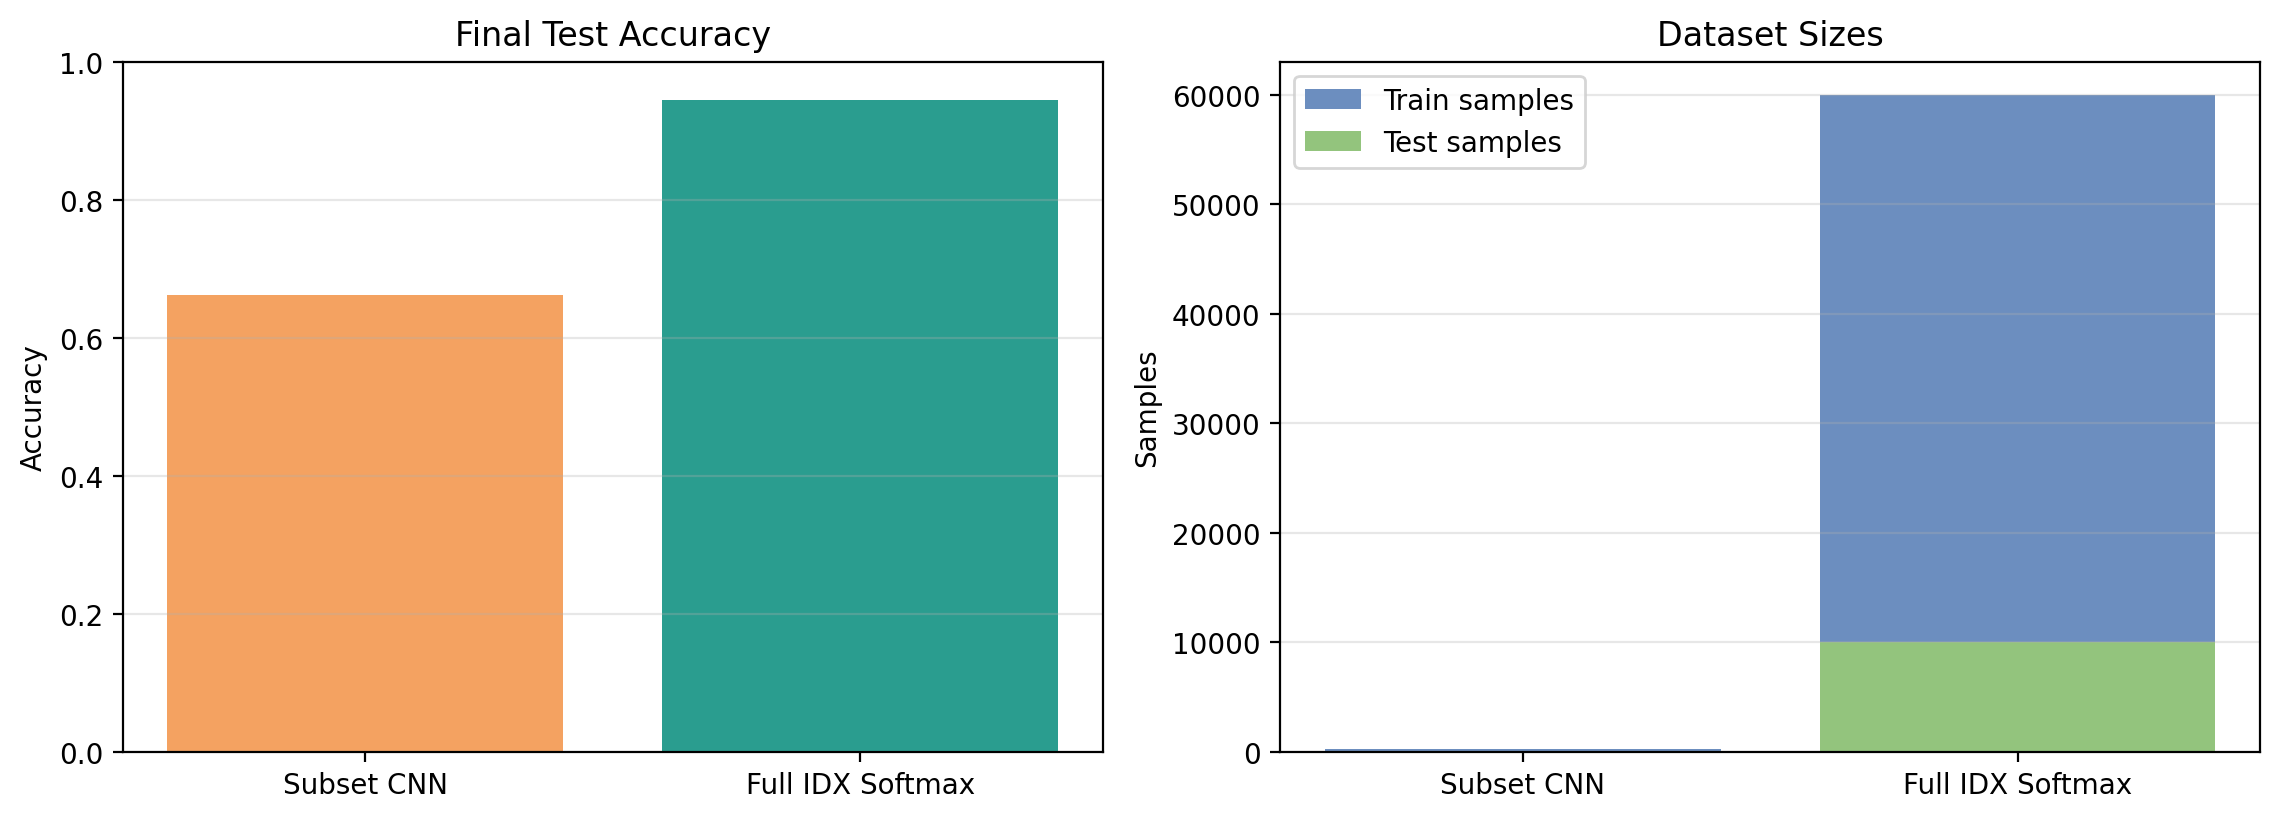
\includegraphics[width=0.9\linewidth]{figures/mnist_experiment_comparison.png}
    \caption{Comparison of final test accuracy and dataset sizes for the subset CNN and the full IDX softmax baseline.}
    \label{fig:comparison}
\end{figure}

The confusion matrices in Figure~\ref{fig:confusion-matrix} reinforce this interpretation. The subset CNN shows substantial class overlap caused by the very small train/test split, whereas the full-dataset softmax baseline produces a much cleaner diagonal structure over the complete 10,000-sample test set. The result should therefore be interpreted as a meaningful software-validation milestone rather than as a competitive benchmark against optimized libraries.

\begin{figure}[htbp]
    \centering
    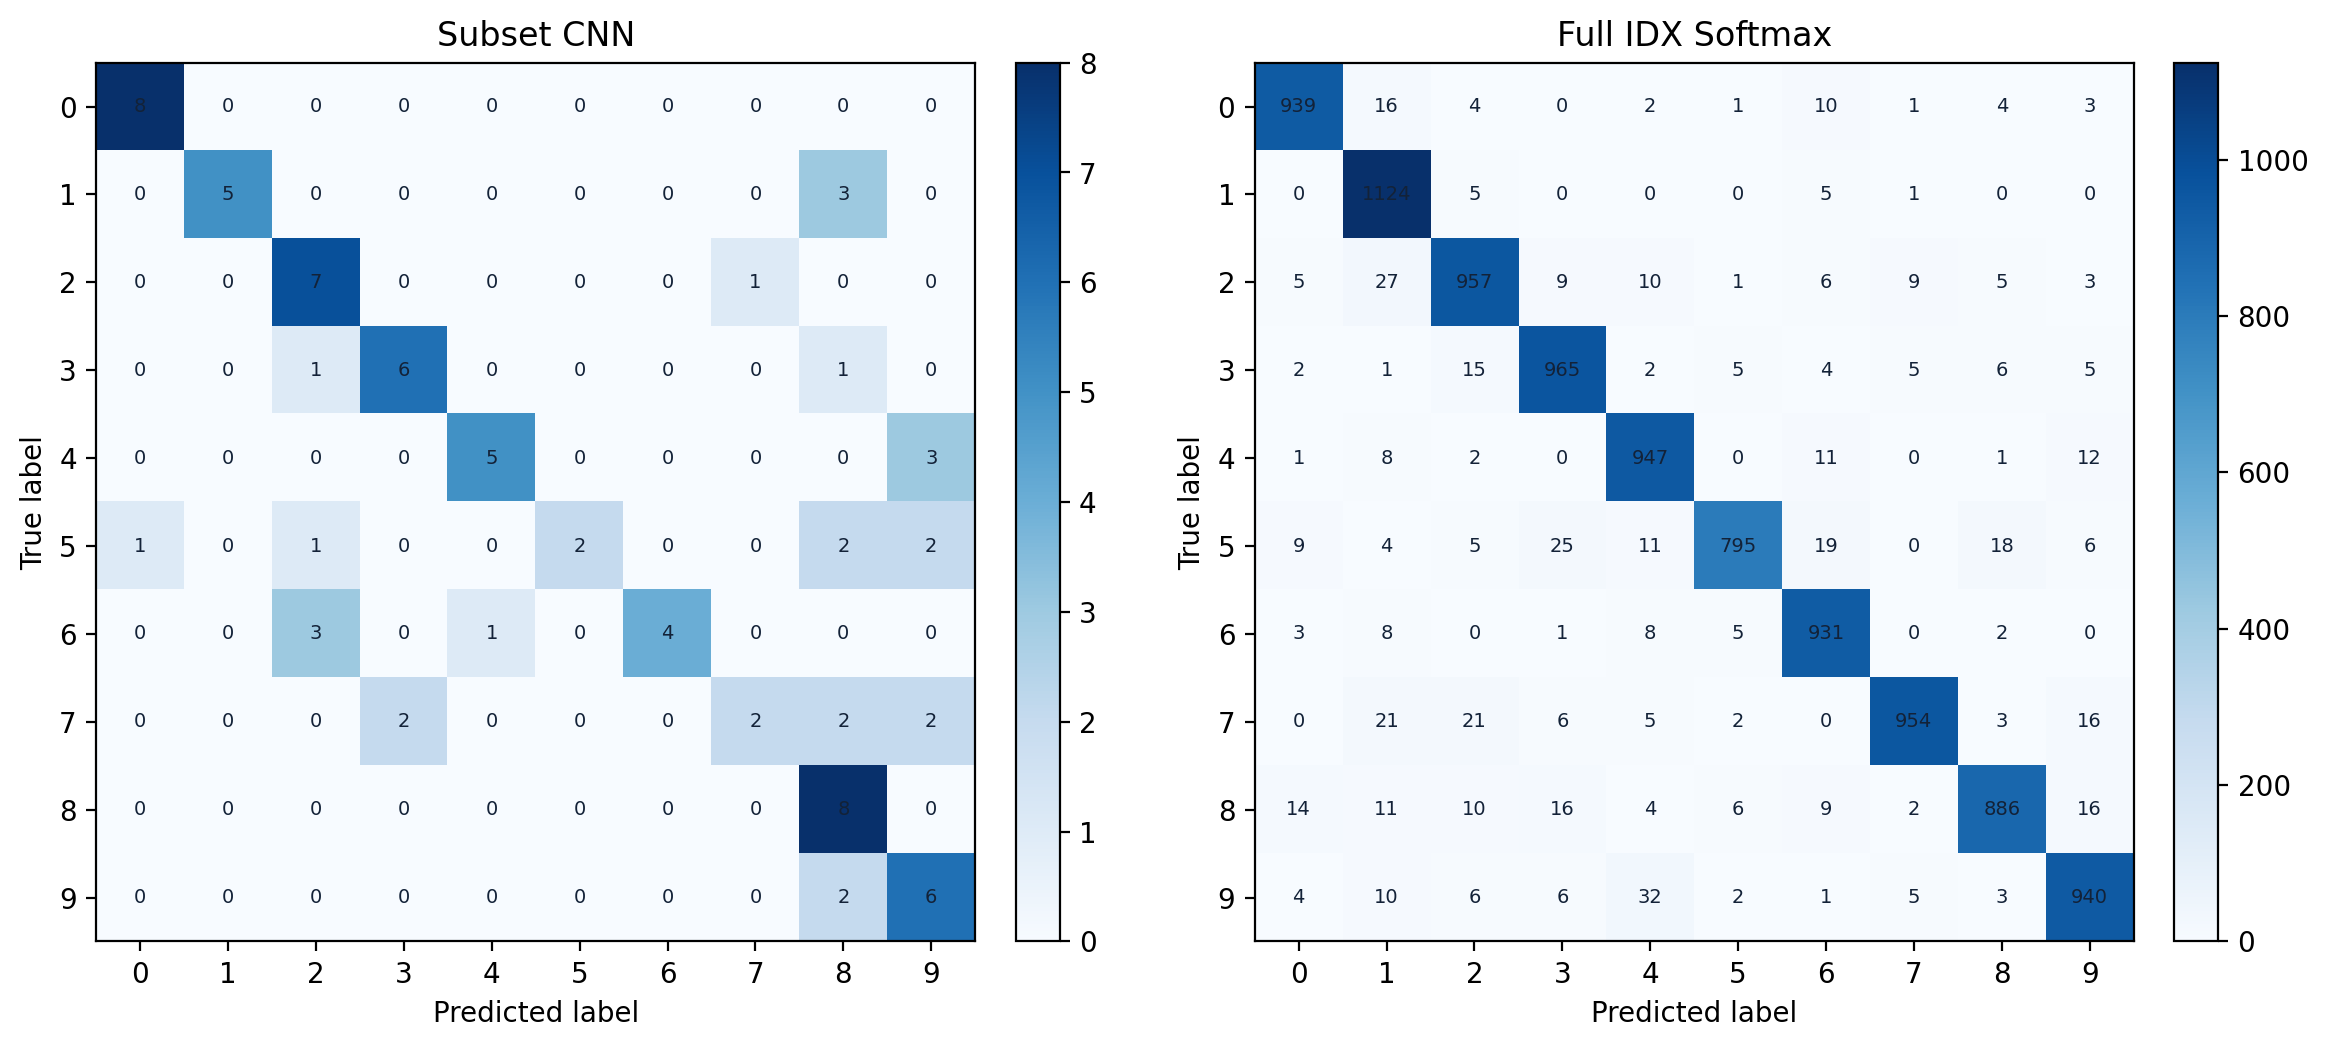
\includegraphics[width=0.72\linewidth]{figures/mnist_confusion_matrix.png}
    \caption{Confusion matrices for the subset CNN and the full-dataset softmax baseline.}
    \label{fig:confusion-matrix}
\end{figure}

\section{Discussion}
The main outcome of the work is software validation rather than state-of-the-art recognition quality. From an implementation perspective, the project now supports the official MNIST binary formats, exposes a lazy loading path that is more RAM-friendly than eagerly duplicating the dataset, implements a softmax output path compatible with multiclass classification, and runs reproducible experiments that generate visual artifacts directly from code. These are meaningful improvements over an earlier draft state with an unfinished parser, missing figures, and an unsuitable linear-output objective for classification.

At the same time, the comparison between the two experiments makes the present trade-off explicit. The convolutional configuration is valuable as a correctness test for the more complex layers, but on a very small subset it does not deliver a stable benchmark result. The full-dataset softmax baseline, by contrast, is simpler architecturally but better matched to the computational limits of a pure Python implementation, and it already exceeds 90\% accuracy on the official MNIST test set. Future work should therefore proceed along two parallel directions: improving the convolutional stack so that larger CNN experiments remain feasible, and extending the training infrastructure with more efficient kernels, richer logging, and stronger numerical tooling. Such improvements would make the library a stronger educational platform and a more convincing research demonstrator.

\section{Conclusion}
This paper documented a pure Python neural network library whose primary value lies in transparency, inspectability, and extensibility. The project was extended with an MNIST IDX parser, corrected dataset shuffling, improved convolutional compatibility, a softmax-based classification head, and a benchmark script that compares a subset CNN with a full-dataset IDX baseline. The full-dataset experiment exceeded 90\% test accuracy on MNIST, while the subset CNN remained useful as a structural validation of the convolutional components. Together, these results provide a concrete and reproducible foundation for further work on optimization, dataset scaling, and experimental methodology. For educational use, this explicit implementation remains valuable precisely because it reveals the details that optimized frameworks intentionally hide.

\begin{acknowledgments}
The author thanks the project mentor for feedback on the experimental scope, publication requirements, and draft preparation process.
\end{acknowledgments}

\bibliography{references}

\end{document}
